\documentclass[12pt,letterpaper]{article}
\usepackage[utf8]{inputenx} %Codificacion del texto (ISO Latin1 encoding)

\usepackage{fancyhdr} %Permite acomodar a tu gusto la parte de arriba y
% abajo del documento
\usepackage[spanish]{babel} %Permite definir el idioma del dcumento
\usepackage{graphicx} %Permite exportar imagenes en formato eps
\usepackage{hyperref}
\usepackage{url} %Tipo de fuente para correos y paginas
\usepackage{pgf}
\usepackage{fleqn}
\usepackage{amssymb}
\usepackage{amsmath}
\usepackage{fancyvrb}
\usepackage{makeidx}
\usepackage{multirow}
\usepackage{colortbl} %Permite colocar colores a las tablas
\usepackage{booktabs}
\usepackage[final]{pdfpages}
%%%%%%%%%%
%Margenes%
%%%%%%%%%%
\parskip 1mm %Espacio entre parrafos

\setlength{\topmargin}{0pt}
\topmargin      0.5cm
\oddsidemargin	0.1cm  % Ancho Letter 21,59cm
\evensidemargin 0.5cm  % Alto  Letter 27,81cm
\textwidth	17cm%15.5cm
\textheight	21.0cm
\headsep	4 mm
\parindent	1.2cm
%%%%%%%%%%%%%%%%%%%%%%
%Estilo del documento%
%%%%%%%%%%%%%%%%%%%%%%
\pagestyle{fancyplain}

%%%%%%%%%%%%%%%%%%%%%%%%%%%%%%%%%%%%%%%%%%%
%Fancyheadings. Top y Bottom del documento%
%%%%%%%%%%%%%%%%%%%%%%%%%%%%%%%%%%%%%%%%%%%
% Recuerde que en este documento la portada del documento no posee
% numeracion, pero de igual manera llamaremos a esa primera pagina la numero
% 1, y la que viene la dos. Esto es para tener una idea de las que
% llamaremos pares e impares
\lhead{Modelado de Procesos de Negocio} %Parte superior izquierda
\rhead{\bf \it Departamento de Informática - UTFSM} %Parte superior derecha
\lfoot{} %Parte inferior izquierda. \thepage indica
% el numero de pagina
\cfoot{} %Parte inferior central
\rfoot{\bf \thepage} %Parte inferior derecha
\renewcommand{\footrulewidth}{0.4pt} %Linea de separacion inferior

\newcommand{\primaria}[1]{
	\textbf{\underline{#1}}
}

\newcommand{\foranea}[1]{
	\textbf{\textsl{#1}}
}

\newcommand{\primyfor}[1]{
	\underline{\foranea{#1}}
}

\makeatletter
\newcommand\subsubsubsection{\@startsection {paragraph}{1}{\z@}%
                                   {-3.5ex \@plus -1ex \@minus -.2ex}%
                                   {1.5ex \@plus.2ex}%
                                   {\normalfont\bfseries}}
\newcommand\subsubsubsubsection{\@startsection {subparagraph}{1}{\z@}%
                                   {-3.5ex \@plus -1ex \@minus -.2ex}%
                                   {1.5ex \@plus.2ex}%
                                   {\normalfont\bfseries}}


\makeatother
\makeindex

\begin{document}
\begin{titlepage}
\title{Modelado de Procesos de Negocio \\ \begin{Large}\it Análisis de Natural Response\end{Large}} 
\author{Victor Gonzalez Rodriguez\\\url{victor.gonzalezr@usm.cl} \\
\and Neil Garcia\\\url{neil.garcia@usm.cl}}
\date{\today}
\maketitle
\begin{abstract}
Lorem ipsum ad his scripta blandit partiendo, eum fastidii accumsan euripidis in, eum liber hendrerit an. Qui ut wisi vocibus suscipiantur, quo dicit ridens inciderint id. Quo mundi lobortis reformidans eu, legimus senserit definiebas an eos. Eu sit tincidunt incorrupte definitionem, vis mutat affert percipit cu, eirmod consectetuer signiferumque eu per. In usu latine equidem dolores. Quo no falli viris intellegam, ut fugit veritus placerat per. Ius id vidit volumus mandamus, vide veritus democritum te nec, ei eos debet libris consulatu. No mei ferri graeco dicunt, ad cum veri accommodare. Sed at malis omnesque delicata, usu et iusto zzril meliore. Dicunt maiorum eloquentiam cum cu, sit summo dolor essent te. Ne quodsi nusquam legendos has, ea dicit voluptua eloquentiam pro, ad sit quas qualisque. Eos vocibus deserunt quaestio ei. Blandit incorrupte quaerendum in quo, nibh impedit id vis, vel no nullam semper audiam. Ei populo graeci consulatu mei, has ea stet modus phaedrum. Inani oblique ne has, duo et veritus detraxit. Tota ludus oratio ea mel, offendit persequeris ei vim. Eos dicat oratio partem ut, id cum ignota senserit intellegat. Sit inani ubique graecis ad, quando graecis liberavisse et cum, dicit option eruditi at duo. Homero salutatus suscipiantur eum id, tamquam voluptaria expetendis ad sed, nobis feugiat similique usu ex. Eum hinc argumentum te, no sit percipit adversarium, ne qui feugiat persecuti. Odio omnes scripserit ad est, ut vidit lorem maiestatis his, putent mandamus gloriatur ne pro. Oratio iriure rationibus ne his, ad est corrumpit splendide. Ad duo appareat moderatius, ei falli tollit denique eos.
\end{abstract}
\end{titlepage}
\newpage
\tableofcontents

\section{Introducción}
Natural Response es una empresa joven, la cual se encarga de procesar y exportar productos naturales extraidos sustentablemente de la flora chilena, tales como el árbol del quillay. Esta empresa ha entrado a un mercado que exige altos estándares de calidad, y ha sabido responder a los requisitos comerciales del exigente mercado de las empresas proveedoras de materias primas y de productos procesados a nivel mundial.\\
Actualmente la empresa se encuentra posicionada dentro de las mejores a nivel mundial abarcando cerca del 80\% del mercado mundial, por lo cual es de interés conocer qué procesos de negocio han llevado al éxito a esta joven empresa. Estudiaremos los procesos de adquisición de productos y de la selección de proveedores; estamos hablando de procesos críticos para la empresa, ya que la mayor parte de sus ingresos se deben a exportaciones al extranjero, los cuales exigen estándares de calidad tales como la norma ISO 9000:2008, la cual asegura la calidad de los productos y de los proveedores de sus implementos de producción. Es decir, el área de estudio de este documento es el área de producción y ventas.\\

\section{Actores y Roles}
\begin{itemize}
\item{\textbf{Gerente de Administración y Recursos Humanos:}} 
\item{Gerente de Planta}
\item{Gerente de Producción}
\item{Jefe de Control de Calidad}
\item{Gerente General}
\item{Gerente/Jefe de Area}
\end{itemize}

\subsection{Estructura Organizacional}
La empresa Natural Response, tiene una estructura jerárquica de responsabilidades, donde existen 7 niveles

\subsubsection{Organigrama de Natural Response}
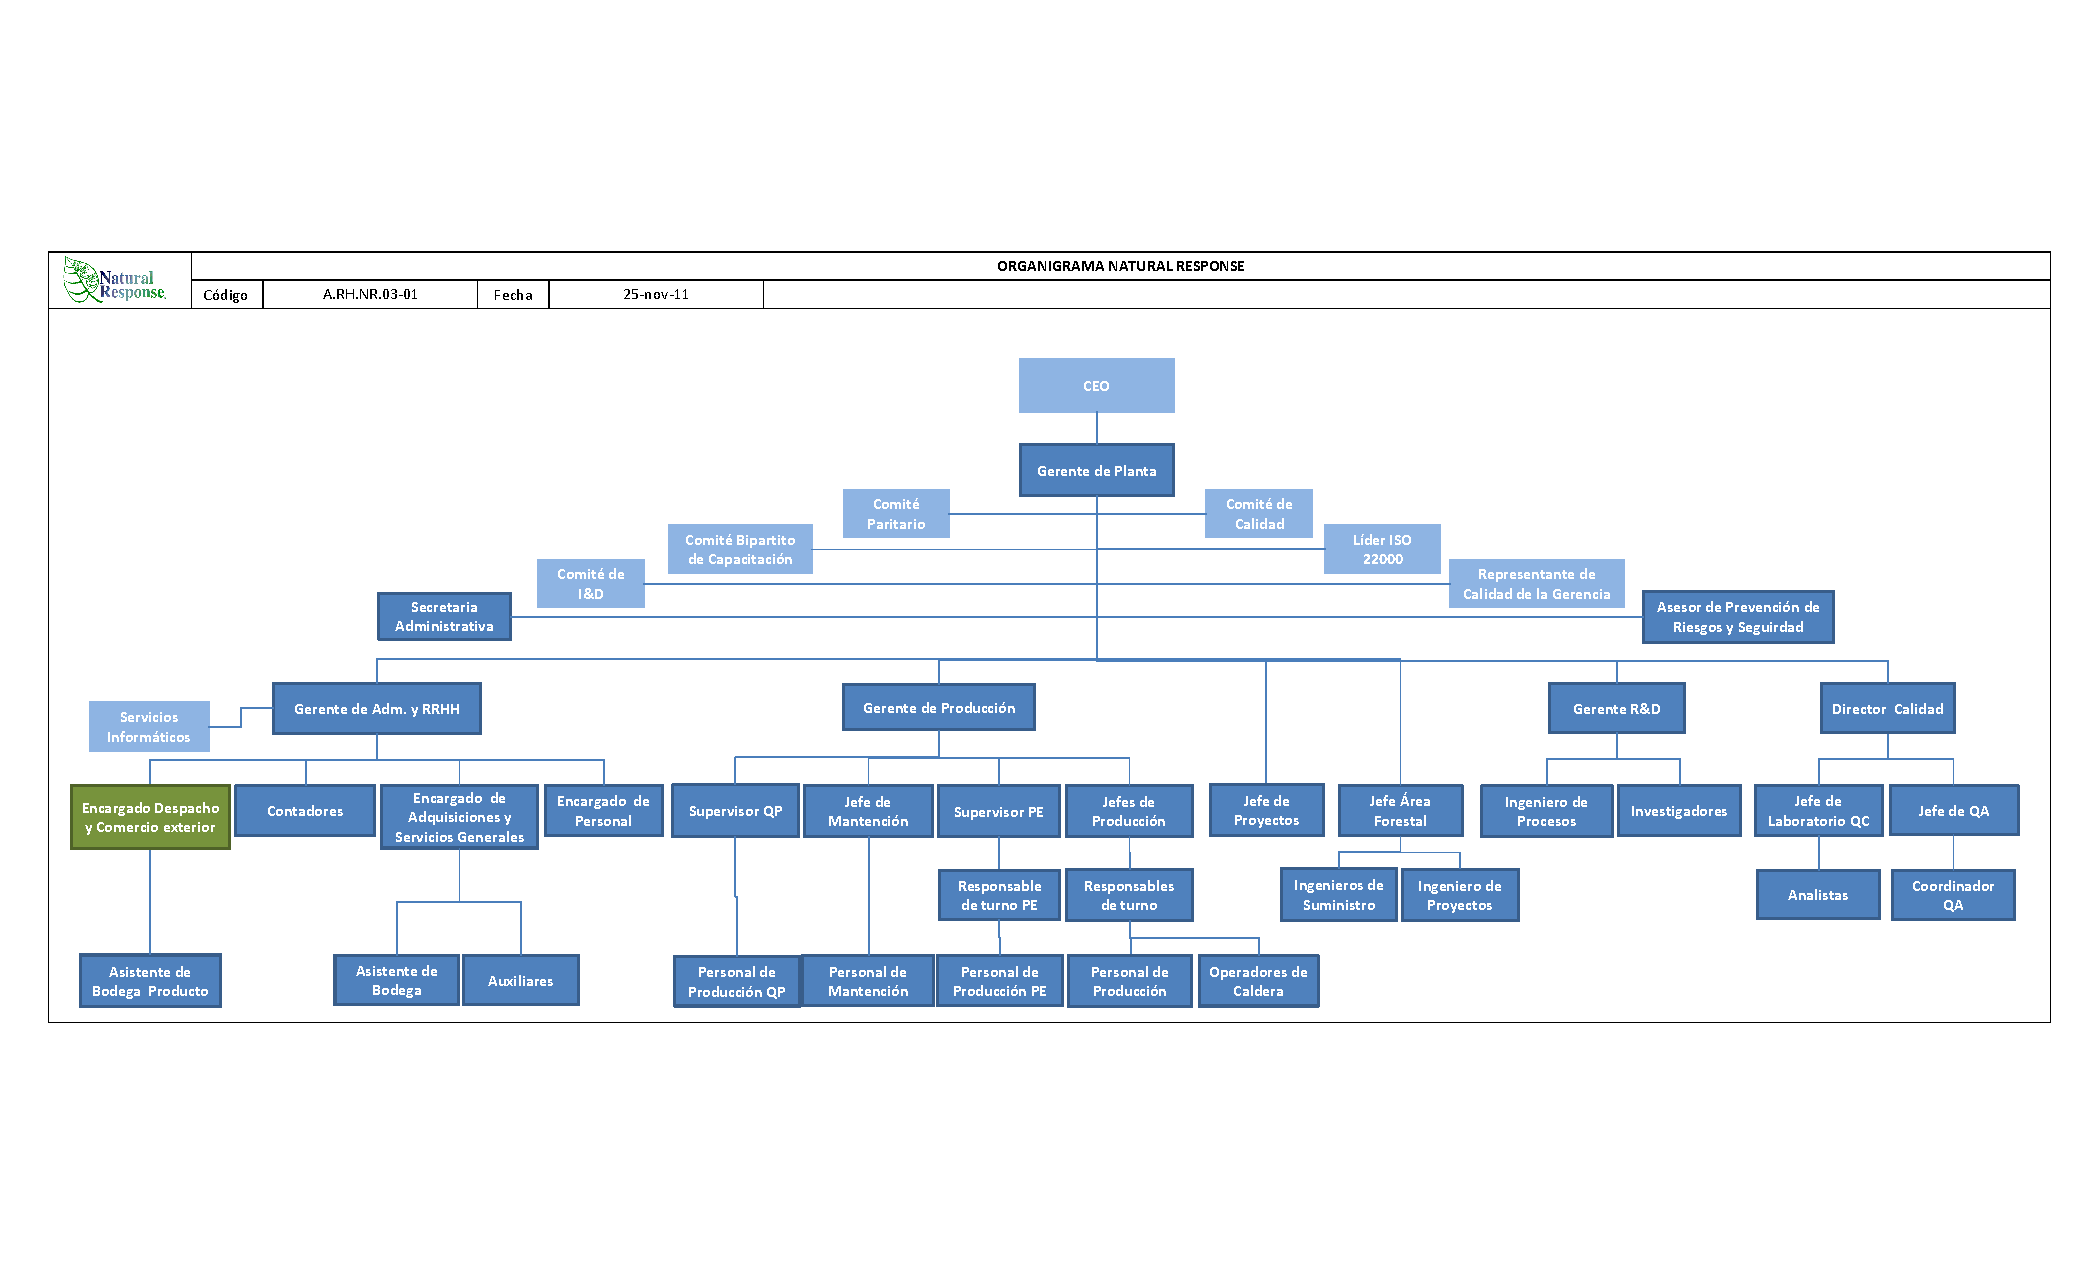
\includegraphics[angle=90,page=1,height=\textheight]{organigrama_nr.pdf}

\subsection{Especificación de los Actores}

\subsection{Descripción de Roles}

\section{Procesos}

\section{Nombre de proceso 1}

\subsection{Definición del Proceso}

\subsubsection{Actores Involucrados}

\subsection{Entradas y Salidas}

\subsection{Indicadores del Proceso}

\subsection{Modelo EPC}

\subsection{Recomendaciones}

\section{Nombre de proceso 2}

\subsection{Definición del Proceso}

\subsubsection{Actores Involucrados}

\subsection{Entradas y Salidas}

\subsection{Indicadores del Proceso}

\subsection{Modelo EPC}

\subsection{Recomendaciones}

\section{Conclusiones}

\subsection{Conclusiones Técnicas}

\subsection{Conclusión de Neil García}

\subsection{Conclusión de Victor Gonzalez}

\section{Recomendaciones}

\section{Referencias}

\end{document} 
